% -*- TeX -*-
\documentclass{beamer}

\usepackage{amsmath}
\usepackage{tikz}
\usetikzlibrary{shapes,calc}

\title{PyLith Modeling Tutorial}
\subtitle{}
\author{Brad Aagaard, Charles Williams, and Matthew Knepley}
\institute{
\includegraphics[scale=0.4]{../../logos/cig_blackfg}}
\date{June 17--19, 2016}


% ---------------------------------------------------- CUSTOMIZATION
\newcommand{\important}[1]{{\bf\color{red}#1}}
\usetheme{CIG}

% --------------------------------------------------------- DOCUMENT
\begin{document}

% ------------------------------------------------------------ SLIDE
\maketitle

% ========================================================== SECTION
\section{Introduction}
\subsection{Agenda}

% ------------------------------------------------------------- LOGO
\logo{
\includegraphics[height=4.5ex]{../../logos/cig_blackfg}}

% ------------------------------------------------------------ SLIDE
\begin{frame}
  \frametitle{Workshop Instructors}
  \summary{}
  
  \begin{center}
    \begin{tabular}{ccc}
      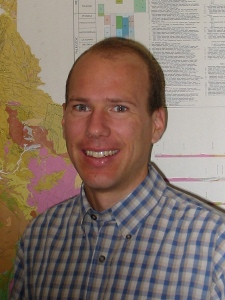
\includegraphics[width=1.2in]{figs/brad} & 
      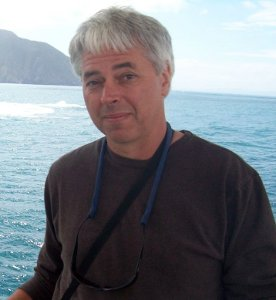
\includegraphics[width=1.2in]{figs/charles} &
      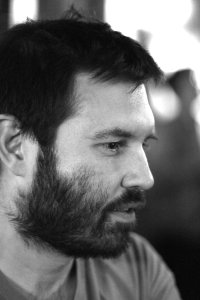
\includegraphics[width=1.2in]{figs/matt} \\
      Brad Aagaard & Charles Williams & Matthew Knepley \\
      USGS & GNS Science & Rice Univ. \\
      Menlo Park, CA & Lower Hutt, NZ & Houston, TX
    \end{tabular}
  \end{center}

\end{frame}


% ------------------------------------------------------------ SLIDE
\begin{frame}
  \frametitle{Overview of Workshop}
  \summary{Agenda posted on geodynamics.org}
  
  \definecolor{yellow}{rgb}{1.0, 1.0, 0.45} % 255/255/115
\definecolor{dkyellow}{rgb}{0.9, 0.9, 0.0} % % 230/230/0

\definecolor{ltorange}{rgb}{1.0, 0.74, 0.41} % 255/188/105
\definecolor{orange}{rgb}{0.96, 0.50, 0.0} % 246/127/0

\definecolor{ltred}{rgb}{1.0, 0.25, 0.25} % 255/64/64
\definecolor{red}{rgb}{0.79, 0.00, 0.01} % 201/0/3

\definecolor{ltpurple}{rgb}{0.81, 0.57, 1.00} % 206/145/255
\definecolor{purple}{rgb}{0.38, 0.00, 0.68} % 97/1/175

\definecolor{ltblue}{rgb}{0.2, 0.73, 1.0} % 51/187/255
\definecolor{blue}{rgb}{0.12, 0.43, 0.59} % 30/110/150

\definecolor{ltltgreen}{rgb}{0.7, 1.00, 0.7} % 96/204/14
\definecolor{ltgreen}{rgb}{0.37, 0.80, 0.05} % 96/204/14
\definecolor{green}{rgb}{0.23, 0.49, 0.03} % 59/125/8
  
\definecolor{dkslate}{rgb}{0.18, 0.21, 0.28} % 47/53/72
\definecolor{mdslate}{rgb}{0.45, 0.50, 0.68} % 114/127/173
\definecolor{ltslate}{rgb}{0.85, 0.88, 0.95} % 216/225/229


\tikzstyle{days} = [rectangle, 
  text centered,
  thin,
  draw=dkyellow!80!black,
  font=\bfseries,
  top color=yellow,
  bottom color=dkyellow]

\tikzstyle{admin} = [rectangle, 
  draw=orange!80!black,
  top color=ltorange!50!white,
  bottom color=orange]

\tikzstyle{handson} = [rectangle, 
  draw=green!80!black,
  top color=ltgreen!20!white,
  bottom color=green]

\tikzstyle{presentation} = [rectangle, 
  draw=blue!80!black,
  top color=ltblue!20!white,
  bottom color=blue]

\tikzstyle{questions} = [rectangle, 
  draw=ltpurple!80!black,
  top color=ltpurple!20!white,
  bottom color=purple!70!white!100]

\begin{center}
\begin{tikzpicture}[scale=0.75, transform shape,
  node distance=2.0em,
  text width=45mm,
  thick]
% Reference points
\coordinate (o1) at (0mm,0mm);
\coordinate (o2) at (+50mm,0mm);
\coordinate (o3) at (+100mm,0mm);

% Days
\node[days] (mon) at ($(o1)$) {Mon};
\node[days] (wed) at ($(o2)$) {Wed};
\node[days] (fri) at ($(o3)$) {Fri};

% Mon
\node[admin, below of=mon] (intro) {Overview};
\node[handson, below of=intro] (refresher) {CUBIT, PyLith, ParaView};
\node[presentation, below of=refresher] (version2) {PyLith 2.0 \& beyond};
\node[questions, below of=version2] (sessionIQ) {Q\&A};

\node[handson, below of=sessionIQ, yshift=-3em] (meshing_2d) {Meshing 2-D};
\node[handson, below of=meshing_2d] (meshing_3d) {Meshing 3-D};
\node[handson, below of=meshing_3d] (meshing_dx) {Cell Size};
\node[questions, below of=meshing_dx] (sessionIIQ) {Q\&A};


% Wed
\node[presentation, below of=wed] (greensfns_intro) {Green's Fns: Overview};
\node[handson, below of=greensfns_intro] (greensfns_2d) {Green's Fns: 2-D};
\node[handson, below of=greensfns_2d] (greensfns_3d) {Green's Fns: 3-D};
\node[questions, below of=greensfns_3d] (sessionIIIQ) {Q\&A};

\node[presentation, below of=sessionIIIQ, yshift=-3em] (solver_intro) {Solvers: Overview};
\node[handson, below of=solver_intro] (solver_linear) {Linear Solvers};
\node[handson, below of=solver_linear] (solver_nonlinear) {Nonlinear Solver};
\node[questions, below of=solver_nonlinear] (sessionIVQ) {Q\&A};


% Fri
\node[presentation, below of=fri] (friction_intro) {Fault Friction: Overview};
\node[handson, below of=friction_intro] (friction_quasi) {Friction: Quasi-static};
\node[handson, below of=friction_quasi] (friction_dyn) {Friction: Dynamic};
\node[questions, below of=friction_dyn] (sessionVQ) {Q\&A};

\node[handson, below of=sessionVQ, yshift=-3em] (parallel_desktop) {Parallel: Desktop};
\node[handson, below of=parallel_desktop] (parallel_cluster) {Parallel: Cluster};
\node[handson, below of=parallel_cluster] (parallel_trouble) {Troubleshooting};
\node[questions, below of=parallel_trouble] (sessionVIQ) {Q\&A};


\end{tikzpicture}
\end{center}


\end{frame}


% ========================================================== SECTION
\subsection{Getting Help}

% ------------------------------------------------------------ SLIDE
\begin{frame}
  \frametitle{Getting Help After the Tutorial Ends}
  \summary{}
 
  \begin{itemize}
  \item Read the PyLith manual
  \item Try to work through the problem on your own
  \item Submit questions to \important{\tt cig-short@geodynamics.org}
    \begin{itemize}
    \item Describe the problem
    \item Send complete error messages
    \item Include the platform you are using, the PyLith version, and
      whether it is a binary package or you built PyLith from source
   \end{itemize}
  \item Subscribe to \important{\tt cig-short@geodynamics.org}
    \begin{itemize}
    \item Answers to most questions will be cc'ed to this email list
    \item Short-term tectonics working group issues are posted here
    \end{itemize}
  \end{itemize}

\end{frame}

% ========================================================== SECTION
\subsection{CIG}

% ------------------------------------------------------------ SLIDE
\begin{frame}
  \frametitle{What is CIG?}
  \summary{Computational Infrastructure for Geodynamics
    ({\tt www.geodynamics.org})}
 
  \vfill

  Objective: Develop, support, and disseminate software for the
  geodynamics community.

  \vfill

  \begin{itemize}
  \item Coordinated effort to develop reusable, well-documented,
    open-source geodynamics software
  \item Strategic partnerships with the larger world of
    computational science and geoinformatics
  \item Specialized training and workshops for both geodynamics and
    larger Earth-science communities
  \end{itemize}

  \vfill
 
  Underlying principle: Earth scientists need help from computational
  scientists to develop state-of-the-art modeling codes

\end{frame}


% ------------------------------------------------------------ SLIDE
\begin{frame}
  \frametitle{CIG: Institution-Based Organization}
  \summary{Educational and not-for-profit organization}
 
  \begin{itemize}
  \item {\bf Open-organization}
    \begin{itemize}
    \item Any institution seeking to collaborate on the development of
      open-source geodynamics software
    \item No cost or size requirements
    \end{itemize}
  \item Current members
    \begin{itemize}
    \item 61 member institutions
    \item 15 foreign affiliates
    \end{itemize}
 \end{itemize}
\end{frame}


% ------------------------------------------------------------ SLIDE
\begin{frame}
  \frametitle{CIG Working Groups}
  \summary{Organized by sub-disciplines}
 
 \begin{itemize}
 \item Short-term tectonics
 \item Long-term tectonics
 \item Mantle convection
 \item Computational seismology
 \item Geodynamo
 \item Magma dynamics
 \end{itemize}

\end{frame}


% ------------------------------------------------------------ SLIDE
\begin{frame}
  \frametitle{Short-Term Tectonics Working Group}
  \summary{}
 
 \vfill
 
 \textbf{Objective}: Simulate crustal deformation across spatial
 scales from $1$ m to $10^3$ km and temporal scales ranging from
 $0.01$ s to $10^5$ years.

 \vfill
 \begin{itemize}
 \item Formed through efforts by Brad Hager and Mark Simons before CIG started
 \item Strong connection to SCEC Stress and Deformation through Time
   (SDOT) focus group
 \item Building connections with SCEC Fault and Rupture Mechanics
   (FARM) focus group
 \end{itemize}
\vfill

\end{frame} 


% ------------------------------------------------------------ SLIDE
\begin{frame}
  \frametitle{CIG Organizational Structure}
  \summary{}
 
  \begin{itemize}
  \item Staff
    \begin{itemize}
    \item Responsible for software development
    \item Director handles day-to-day decisions
    \end{itemize}
  \item Science Steering Committee
    \begin{itemize}
    \item Voice of geophysics community
    \item Prioritizes the competing needs of all sub-disciplines
    \end{itemize}
  \item Executive Committee
    \begin{itemize}
    \item Primary decision-making body
    \item Approves SSC recommendations and contractual arrangements
    \end{itemize}
  \item Member institution representatives
    \begin{itemize}
    \item Vote on membership applications and bylaws
    \end{itemize}
  \item Community members
    \begin{itemize}
    \item Collaborate with staff to develop software
    \end{itemize}
  \end{itemize}

\end{frame}

% ------------------------------------------------------------ SLIDE
\begin{frame}
  \frametitle{CIG Activities}
  \summary{}

  \begin{itemize}
  \item Software development: primary activity
  \item Workshops
    \begin{itemize}
    \item Sponsors workshops organized by one or more working groups
    \item Holds workshops focusing on scientific computing and geodynamics
    \end{itemize}
  \item Training in use of CIG software
    \begin{itemize}
    \item Tutorials at workshops
    \item Specialized training sessions (like this one)
    \end{itemize}
  \item Web site: {\tt geodynamics.org}
    \begin{itemize}
    \item Distribution of software and documentation
    \item Mailing lists for each working group
    \item Wiki-like web pages for community involvement
    \end{itemize}
  \end{itemize}
 
\end{frame}


% ------------------------------------------------------------ SLIDE
\begin{frame}
  \frametitle{CIG Software}
  \summary{}

  \vfill
  \begin{center}
    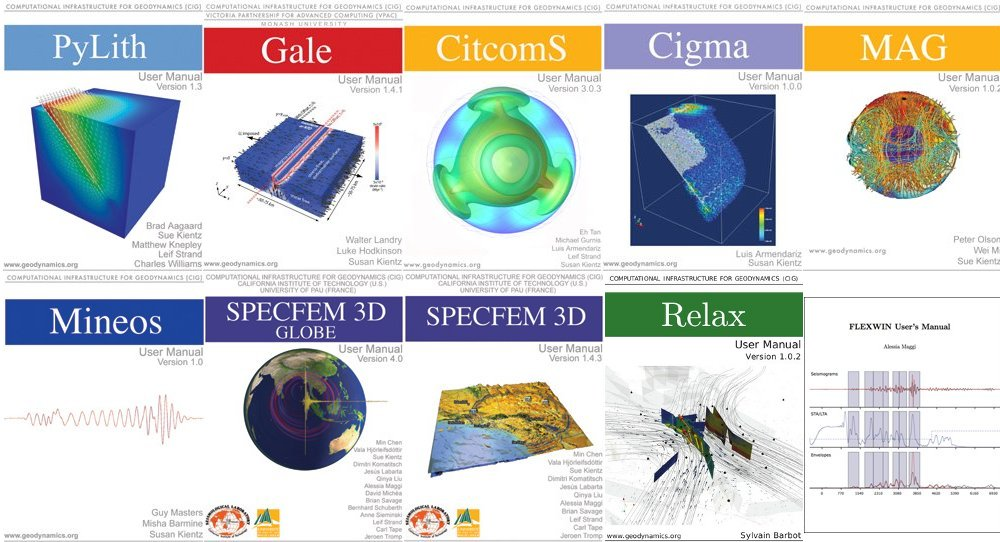
\includegraphics[width=4.5in]{figs/covers}
  \end{center}
  \vfill

\end{frame}

% ------------------------------------------------------------ SLIDE
\begin{frame}
  \frametitle{CIG Software for Crustal Deformation}
  \summary{}

  \begin{itemize}
  \item Relax
    \begin{itemize}
    \item Solves 3-D problems associated with earthquake faulting and
      quasi-static viscoelastic deformation
    \item Short-term tectonics in a homogeneous half-space where
      geometry does not change significantly
    \end{itemize}
  \item PyLith
    \begin{itemize}
    \item Solves 2-D and 3-D problems associated with earthquake
      faulting and quasi-static and dynamic viscoelastic deformation
    \item Short-term tectonics where geometry does not change
      significantly
    \end{itemize}
  \item Gale
    \begin{itemize}
    \item Solves problems in orogenesis, rifting, and subduction,
      including free surfaces with coupling to surface erosion models
    \item Long-term tectonics where geometry changes significantly
    \end{itemize}
 
  \item Virtual Quake
    \begin{itemize}
    \item Boundary element code that simulates earthquakes on fault systems based on stress interactions
    \end{itemize}
  \end{itemize}
 
\end{frame}

 
% ======================================================================
\end{document}


% End of file
